\chapter{Z Background Estimation}

We describe here two methods of estimating $Z\rightarrow\ell\ell$ backgrounds in our strong SUSY regions. The first method relies on the statistical manipulation of data-driven photon+jets backgrounds, and has been used in our previous analyses. We describe this method, and show that it is ill-suited to our current analysis due to violation of several underlying method assumptions. The second method we describe, based on the scaling of Z Monte Carlo samples to a \mindphijm\ control region for each signal and validation region, is the one we use for our current search. We show that this method replicates important features accurately, and is robust to theory systematic variations.

\section{Photon Method}

The photon+jets method is one which has been used before in both ATLAS and CMS~\cite{blah}, including in one of our previous analyses~\cite{blah}. In this method, we take photon+jets events from data and perform statistical manipulation to make them look like Z+jets events (Figure~\ref{fig:photon_to_Z}).

\begin{figure}[htbp]
    \centering
    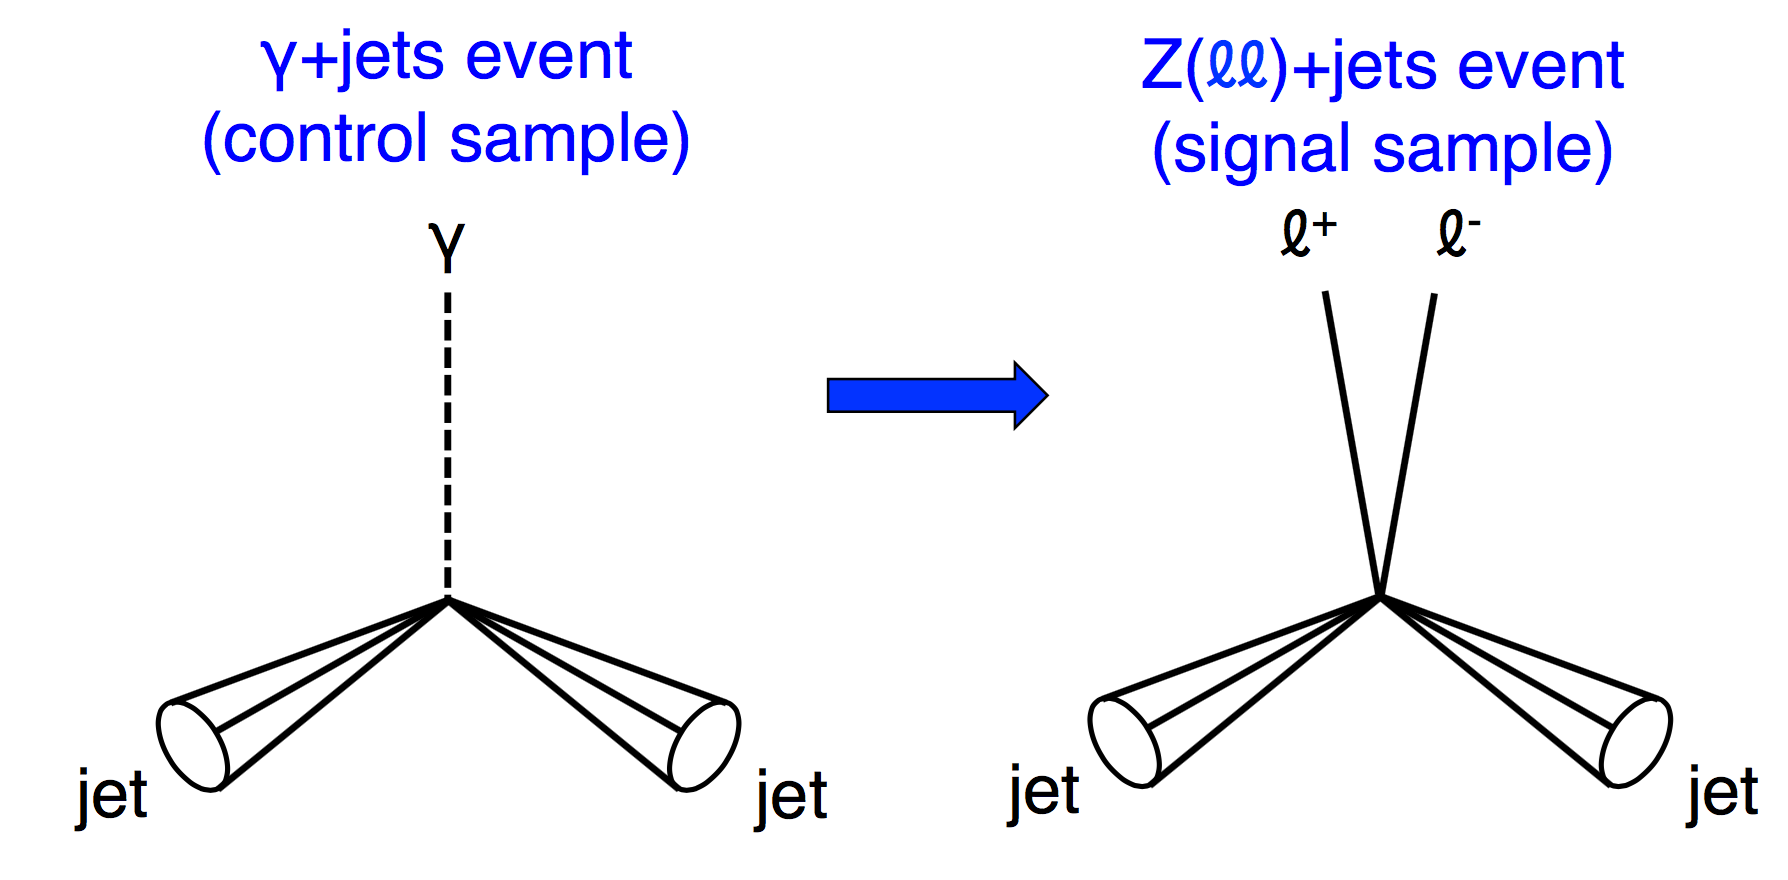
\includegraphics[width=\textwidth]{Images/SUSY/photon_to_Z.png}
    \caption{A photon+jets event is made to resemble a Z+jets event by treating the photon as a Z boson of the same momentum, and by splitting it into two leptons.}
    \label{fig:photon_to_Z}
\end{figure}

The reason we do this is overcome limitations in QCD modelling in jets. That is, since most of the \MET\ in Z+jets events comes from the jets, and not from the Z or its lepton daughters, any analysis which involves \MET\ would benefit from using data-driven methods of estimating this particular background.

In this method, we can take a photon+jets event and treat the photon as a Z boson of the same \pt. We first "pseudo-split" the photon into two leptons. Second, we perform smearing adjustments on the leptons to simulate their relative measurement uncertainties. Finally, we scale the entire photon+jets \pt\ distribution to match the Z+jets \pt\ distribution.

\subsection*{Splitting}

To split the photon into two leptons, we first boost into the rest frame of the photon and perform the decay via a uniform angle sampling on the unit sphere. We then boost the daughter leptons back to the lab frame. In theory, this would allow us to replicate the lepton distributions in our Z+jets background.

However, here we run into our first problem. There are differences in the $\eta$ distributions of photons and Z bosons (Figure~\ref{fig:Z_photon_eta}). As well, there are $\eta$ acceptance distributions for each type of lepton. As such, we have to perform a reweighting in lepton $\eta$ to get the photon "pseudo-split" leptons to match up. However, this is made more difficult by the $|\eta|<2.37$ requirement on photons, as well as the $\eta$ acceptance gaps.

\begin{figure}[htbp]
    \centering
    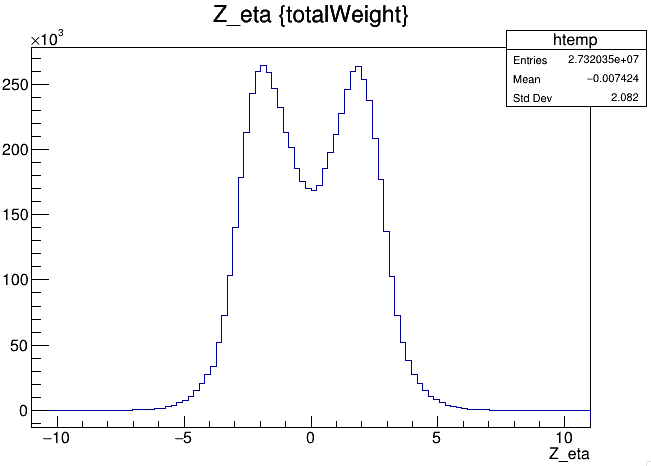
\includegraphics[width=0.45\textwidth]{Images/SUSY/Z_eta.png}
    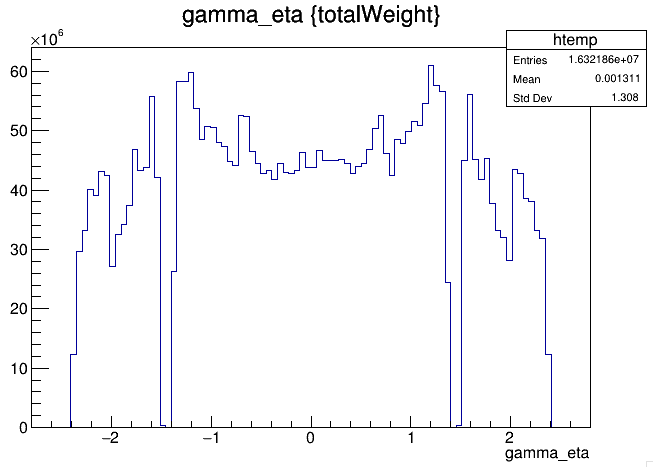
\includegraphics[width=0.45\textwidth]{Images/SUSY/photon_eta.png}
    \caption{Z $\eta$ distribution (left) vs. photon $\eta$ distribution.}
    \label{fig:Z_photon_eta}
\end{figure}

By having to use low-$\eta$ photons to simulate high-$\eta$ Z+jets events, we get slight unavoidable differences in lepton distributions. These problems caused some issues in final \MET\ distributions, since the leptons were used to perform \MET\ smearing (as will be described next).

\subsection*{Smearing}

The resolution smearing step is to account for the fact that photons and leptons have different measurement resolutions within our detector. In particular, there is significant mismeasurement of muons at high \pt, which produces a contribution to \MET\ in the propagation direction of the muon. Though most \MET\ in our Z/$\gamma$+jets events is taken to be coming from the jets, these leptonic contributions cause an effect which must be corrected for.

To simplify calculations, we treat lepton propagation as mostly being in the direction of Z/$\gamma$ propagation. Thus our smearing method only affects \MET\ in the direction parallel to the direction of Z/$\gamma$ propagation (\METl), and not in the transverse direction (\METt). To apply smearing, we look at \METl\ in slices of \pt\ for both photon and Z events in MC. For each bin, we calculate the differences in mean and standard deviation for the photon and Z distributions.

For electrons we apply a shift in mean \METl\ for each event, and for muons we apply both a shift in mean and an additional smearing in resolution based on sampling from a Gaussian of the given standard deviation. Comparisons of photon and Z \METl\ distributions after smearing in various \pt\ slices can be seen in Figure~\ref{fig:Z_photon_eta}.

\begin{figure}[htbp]
    \centering
    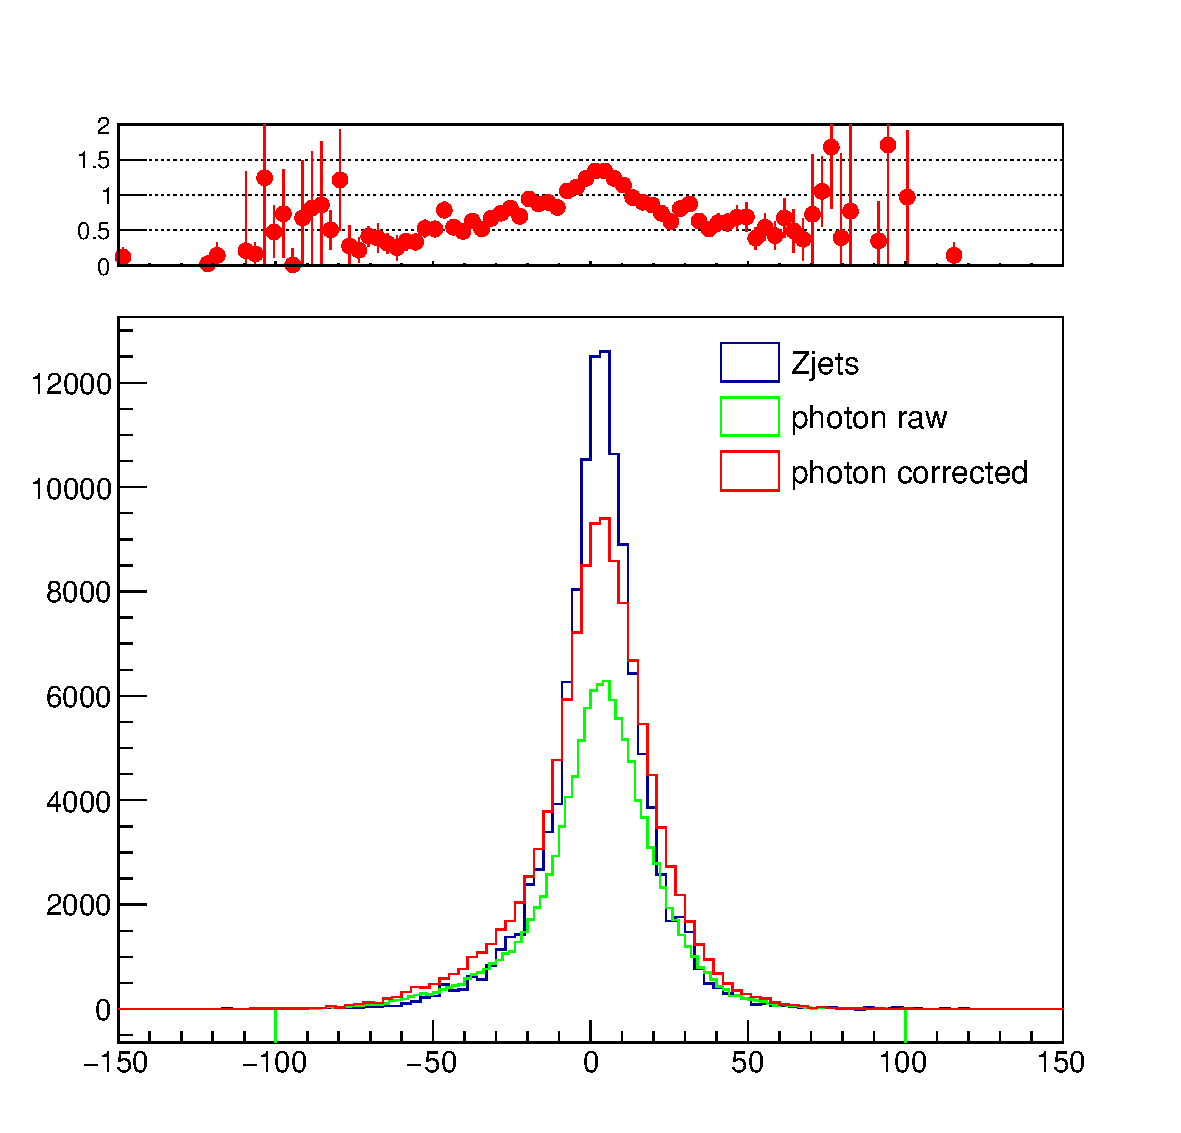
\includegraphics[width=0.45\textwidth]{Images/SUSY/METl_bin_5.pdf}
    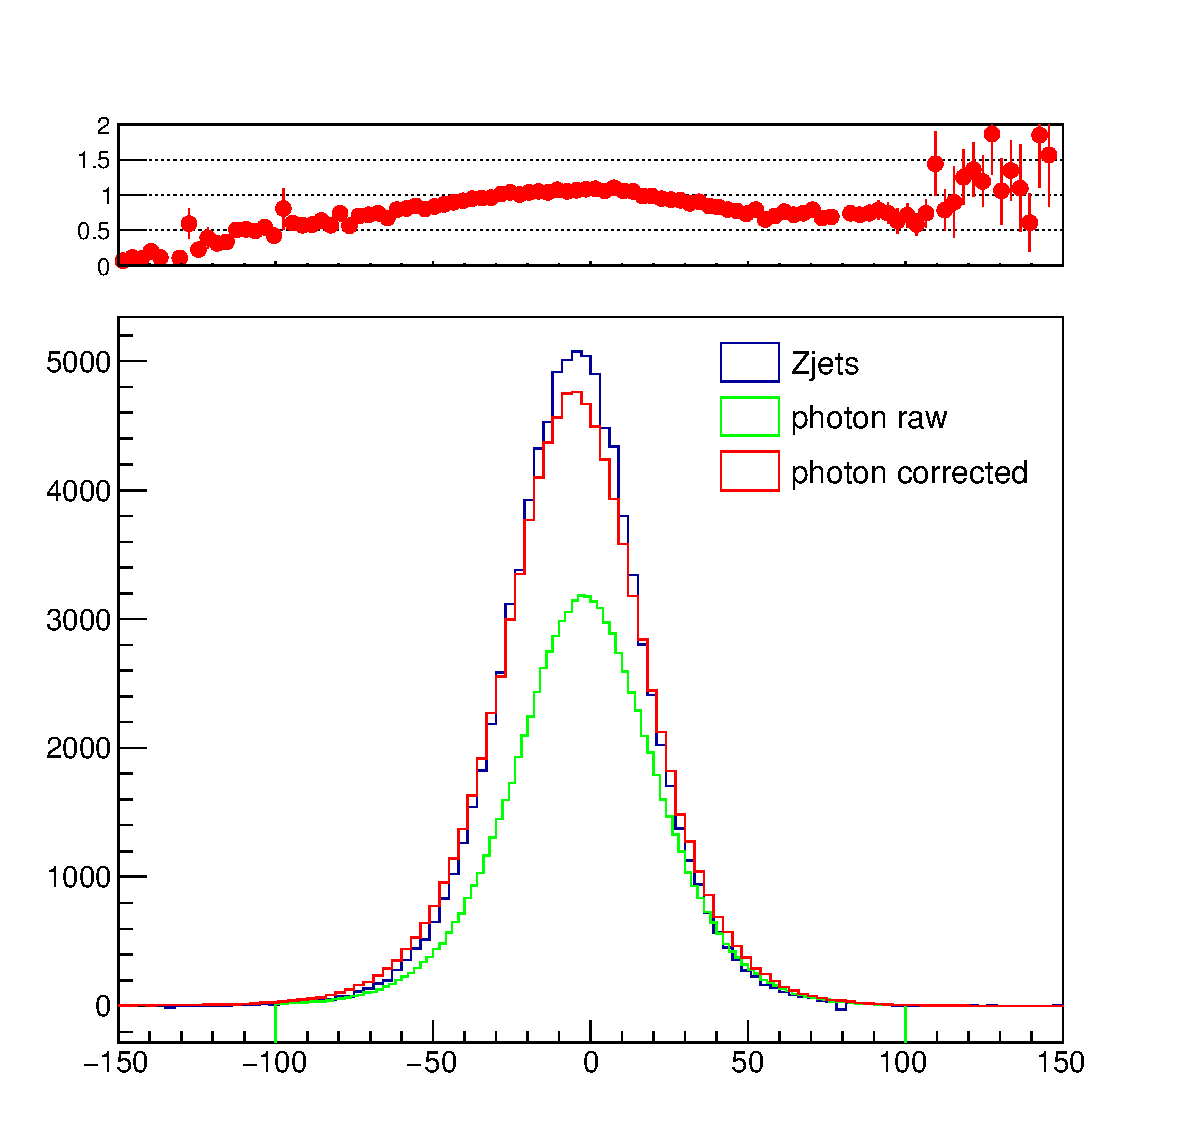
\includegraphics[width=0.45\textwidth]{Images/SUSY/METl_bin_16.pdf}
    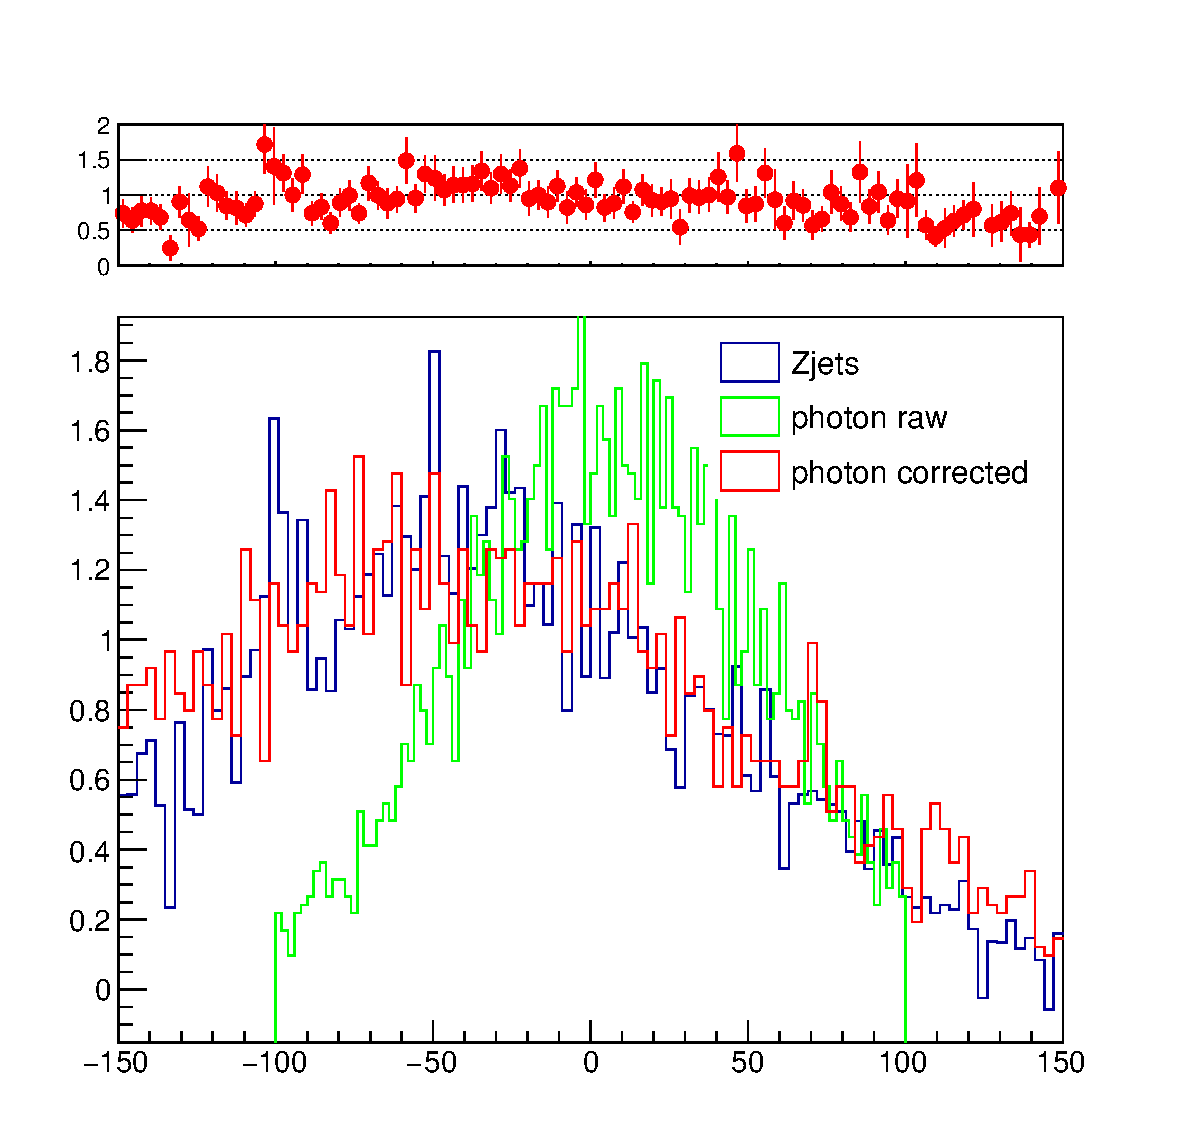
\includegraphics[width=0.45\textwidth]{Images/SUSY/METl_bin_21.pdf}
    \caption{\METl\ comparisons between Z+jets (in the $\mu\mu$ channel) and smeared photon+jets events in a low-\pt\ bin (left), a medium-\pt\ bin (right), and a high-\pt\ bin (bottom). Scaling has been applied to smeared photons.}
    \label{fig:Z_photon_eta}
\end{figure}

These \pt-binned \METl\ comparisons reveal a problem. Though \METl\ is replicated well at high \pt, turning a photon distribution that looked nothing like the Z distribution into something fairly close, the effect is not so good at low \pt. In fact, at low \pt\ we see that the photon resolution started off worse than the muon resolution, violating one of the assumptions of our method. There, the smearing method allowed us to mean-shift to better match the Z+jets \METl\ distribution, but could not simulate the required improvement in resolution.

The overall result of the smearing method can be seen in Figure~\ref{fig:Z_photon_eta_total}. We see that though the photon \METl\ distribution has improved, it still does not match well with the Z+jets distribution. In particular, there is a skew issue which comes from the facts that \METl\ means shift leftward as \pt\ increases, and that smearing performs worse at low \pt. This problem ended up causing mismodeling issues with the \MET\ variables.

\begin{figure}[htbp]
    \centering
    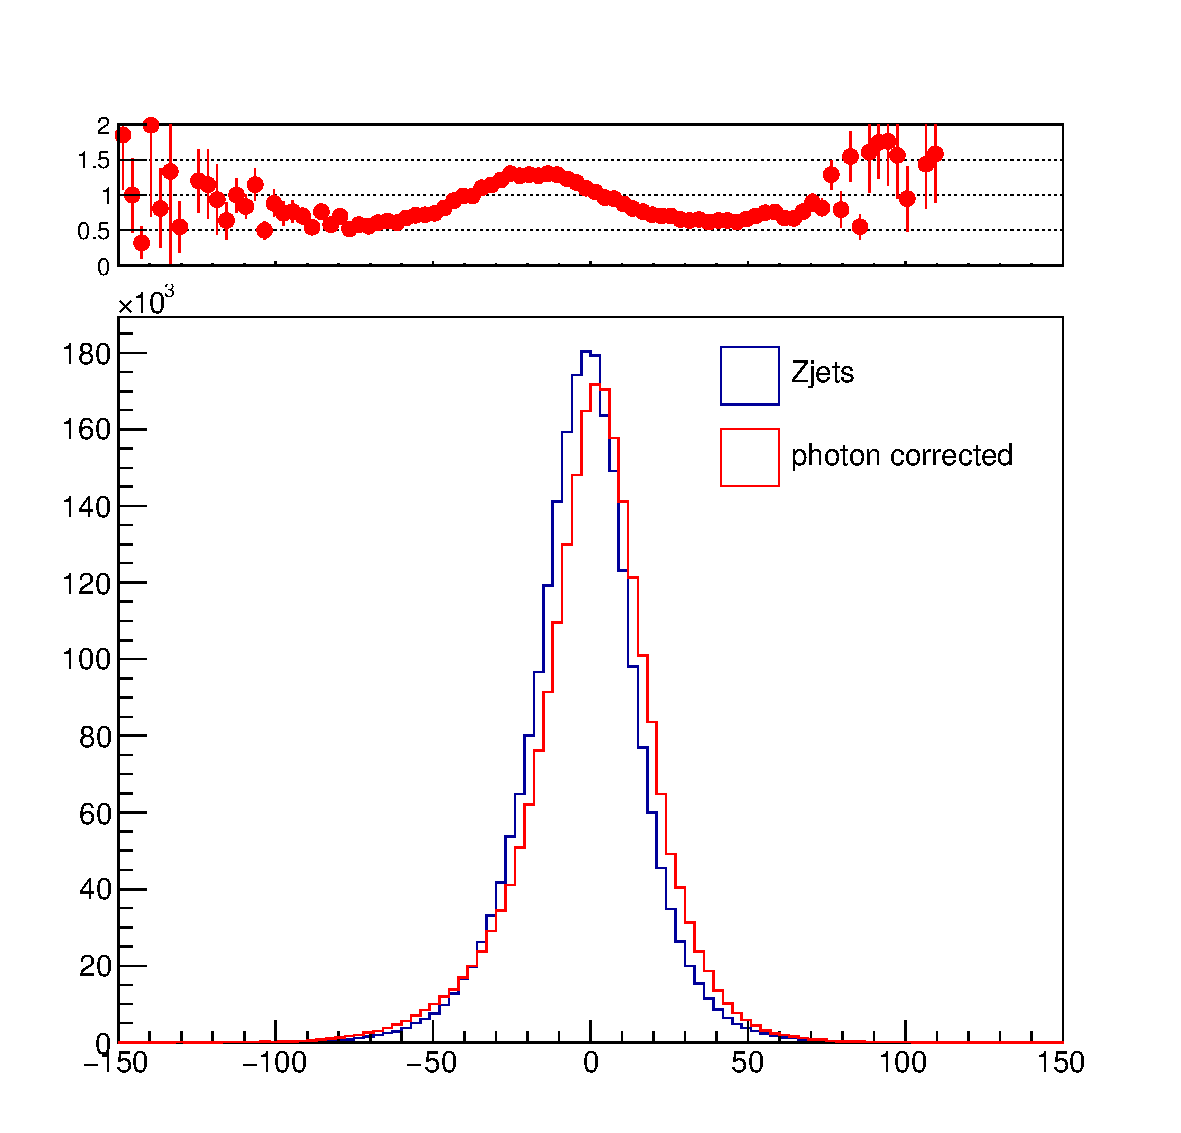
\includegraphics[width=0.45\textwidth]{Images/SUSY/METl_total.pdf}
    \caption{\METl\ comparisons between all Z+jets and smeared photon+jets events.}
    \label{fig:Z_photon_eta_total}
\end{figure}

\subsection*{Reweighting}

Next, we take into account the fact that photon and Z processes are produced with different \pt\ distributions. We correct for this by reweighting photon events in \pt\ bins in order to match the distribution seen in Z events. To do this, we look at an inclusive region (<INSERT REGION>) and apply a scaling factor for each photon event based on yields in the pT slices. Comparisons of photon vs. Z pT (Ptll) distributions both before and after reweighting are shown in Figure~\ref{fig:reweighting}.

\begin{figure}[hbtp]
    \centering
    %\includegraphics{}
    \caption{Caption}
    \label{fig:reweighting}
\end{figure}

However, this leads to our third problem. We see in the plot that the photon and Z \pt\ ranges are not the same. This is due to different availabilities of photon and Z triggers. Lacking the low-\pt\ photon information means that a lot of the soft lepton events would be inaccurately modelled by this method.

\subsection*{Examining Other Assumptions}

[MET not all from jets]

[show MET feature plots]

\section{Z MC Method}

Due to all of the problems listed in the last section, we decided to take a look at Z MC again. Luckily, it appeared that with recent Monte Carlo sample generation updates, many of the problems previously seen with QCD modelling were no longer an issue. Various feature checks revealed that Z MC modelled \MET\ variables well.

\subsection*{Z Feature Checks}

\subsection*{dPhi Scaling Method}

\subsection*{Yield Tables}

\subsection*{Systematic Tables}

Here we compare two methods for obtaining theory systematic uncertainties for the Z background. First we have the \mindphijm method, as described in the body of the paper, and for which the Strong region systematics uncertainties are reproduced in Table~\ref{tab:ZMC_ratio_systematics_rep}. Second, we have the uncertainties in yield which we would obtain just from taking the differences in Z MC yield for each region. This is shown in Table~\ref{tab:ZMC_yield_systematics}.

The yield systematics are quoted by using the maximum \mll bin yield difference in each region, using the binning scheme as described in the body of our paper. If the highest bin yield difference is an outlier (at least $10\%$ higher than the second-highest difference), then we quote the second-highest difference instead. We see that this method produces theory systematic uncertainties which are much higher than those obtained for the \mindphijm method. We demonstrate this difference by looking at the \mindphijm shapes in three regions, SRC (Figure~\ref{fig:mindphijm_SRC}), SRLow (Figure~\ref{fig:mindphijm_SRLow}), and SRHigh (Figure~\ref{fig:mindphijm_SRMed}). In these plots we show the nominal \mindphijm distribution against the scale and PDF variations with the largest differences in yield uncertainty. These plots demonstrate that though total Z MC yield is strongly influenced by systematic variations, the \mindphijm distribution shape is relatively unaffected. Thus our \mindphijm ratio method is robust to these systematic changes.

\begin{table}
\caption{Z MC dPhi Ratio Systematic Uncertainties}
\begin{center}
\begin{tabular}{c|c|c}
region & scale uncertainty & PDF uncertainty \\
\hline
SRC & 0.410 & 0.068 \\
SRLow & 0.058 & 0.001 \\
SRMed & 0.014 & 0.010 \\
SRHigh & 0.042 & 0.019 \\
SRLowZ & 0.035 & 0.007 \\
SRMedZ & 0.017 & 0.008 \\
SRHighZ & 0.006 & 0.014 \\
VRC & 0.124 & 0.088 \\
VRLow & 0.044 & 0.011 \\
VRMed & 0.038 & 0.003 \\
VRHigh & 0.013 & 0.006 \\
VRLowZ & 0.015 & 0.010 \\
VRMedZ & 0.010 & 0.003 \\
VRHighZ & 0.026 & 0.017 \\
\end{tabular}
\end{center}
\label{tab:ZMC_ratio_systematics_rep} 
\end{table}

\begin{table}
\caption{Z MC Yield Systematic Uncertainties}
\begin{center}
\begin{tabular}{c|c|c}
region & scale uncertainty & PDF uncertainty \\
\hline
SRC & 0.545 & 0.078 \\
SRLow & 0.542 & 0.048 \\
SRMed & 0.464 & 0.046 \\
SRHigh & 0.473 & 0.136 \\
SRLowZ & 0.527 & 0.035 \\
SRMedZ & 0.492 & 0.037 \\
SRHighZ & 0.471 & 0.046 \\
VRC & 0.651 & 0.052 \\
VRLow & 0.597 & 0.083 \\
VRMed & 0.475 & 0.026 \\
VRHigh & 0.438 & 0.026 \\
VRLowZ & 0.480 & 0.029 \\
VRMedZ & 0.471 & 0.019 \\
VRHighZ & 0.449 & 0.020 \\
\end{tabular}
\end{center}
\label{tab:ZMC_yield_systematics} 
\end{table}

\begin{figure}[tbhp]
\centering
%\includegraphics[width=0.8\textwidth]{figures/ZMC/systematics/SRC.png}
\caption{
\mindphijm shape for nominal Z MC in the SRC region, compared with shapes for scale and PDF systematics with the largest differences in yield.
}
\label{fig:mindphijm_SRC} 
\end{figure} 

\begin{figure}[tbhp]
\centering
%\includegraphics[width=0.8\textwidth]{figures/ZMC/systematics/SRLow.png}
\caption{
\mindphijm shape for nominal Z MC in the SRLow region, compared with shapes for scale and PDF systematics with the largest differences in yield.
}
\label{fig:mindphijm_SRLow} 
\end{figure} 

\begin{figure}[tbhp]
\centering
%\includegraphics[width=0.8\textwidth]{figures/ZMC/systematics/SRMed.png}
\caption{
\mindphijm shape for nominal Z MC in the SRMed region, compared with shapes for scale and PDF systematics with the largest differences in yield.
}
\label{fig:mindphijm_SRMed} 
\end{figure} 